\Chapter{Predchádzajúce riešenia 2}{Techniky vizualizácie vo verifikácii}
\label{chap:prevvis}

\section{Bodový graf}
\label{sec:scatterplot}
Najjednoduchším spôsobom ako analyzovať vzťah dvoch náhodných premenných je \textit{bodový graf}, ktorý je inak nazývaný aj \textit{korelačný diagram} a známy je tiež pod svojim anglickým pomenovaním \textit{scatter plot}. Bodový graf je vhodný na štúdium kolerácie dvoch premenných a taktiež je výborný pri odhaľovaní takzvaných \mbox{\textit{outlier}-ov}, teda hodnôt, ktoré sa nejakým spôsobom výrazne odlišujú od tých ostatných. Taktiež nám nepriamo podáva správu o distribúcii hodnôt, čo však pri ich veľkom počte môže byť skreslené, keďže sa body začnú postupne prekrývať, a tak nemožno určiť v akej oblasti je viacej, či menej bodov. Tento jav sa nazýva \textit{overplotting}.


\subsection{Konštrukcia bodového grafu}
Skonštruovanie bodového grafu je veľmi jednoduché a aj preto je často používaným prostriedkom na vizualizáciu. Na svoju konštrukciu využíva karteziánsku sústavu súradníc. Dve náhodné premenné, ktoré chceme porovnať, vizualizujeme tak, že spravíme zobrazenie jednej premennej na \mbox{$ x $-ovú} súradnicovú os a zobrazenie druhej premennej na \mbox{$ y $-ovú} os. Následne v danom bode nakreslíme určený symbol, čo zvyčajne býva čierna bodka alebo krúžok. 
Na obrázku \ref{fig:scattervsqq}a) vidíme príklad výsledného bodového grafu, ktorý vznikne takýmto postupom.

Bodový graf ponúka mnoho spôsobov, ako pridať ďalší rozmer informácie do vizualizácie. Môžeme zvoliť odlišnú súradnicovú sústavu, čím veľmi jednoducho vytvoríme napríklad 3D bodový graf pre trojrozmerné dáta. Ďalšou možnosťou rozšírenia je zmena vykresľovaného symbolu, ktorému môžme nastavovať rôzne parametre, do ktorých možno zakódovať nové informácie. Zvyčajne sú týmito parametrami farba, \mbox{alfa-transparencia} \cite{SolutionToOverplotting}, veľkosť \cite{Viegas}, tvar \cite{GenSensScatterplot, EnhanceScatterplot} a podobne. Tieto modifikácie si v komunite vizuálnej analýzy vyslúžili aj vlastné názvy a teoretické zázemie, avšak v našej práci sa týmto druhom diagramov nebudeme venovať.

\subsection{Kantil-kvantil graf}
\label{subsec:qqplot}
Dôležitou a často využívanou variáciou pre bodový graf je \textit{kvantil-kvantil graf}, skrátene \textit{\mbox{Q-Q} graf} (Q z anglického \textit{quantil}). Jediným rozdielom medzi bodovým grafom a \mbox{Q-Q} grafom je, že zatiaľ, čo bodový graf vizualizuje surové dáta, \mbox{Q-Q} graf zobrazuje iba kvantily z oboch dátových množín. 

Kvantilmi sú hodnoty, ktoré rozdeľujú usporiadanú dátovú množinu na niekoľko rovnako veľkých častí. Pre jednu dátovú množinu je $ (q - 1) $ $ q $-kvantilov. Najznámejším príkladom je \mbox{2-kvantil}, ktorý sa nazýva medián. Ďalšími bežnejšie používanými sú \mbox{4-kvantily}, \mbox{10-kvantily} a \mbox{100-kvantily}, čo sú vlastne kvartily, decily a percentily. 

To, čo sa zvyčajne robí pri \mbox{Q-Q} grafe je, že sa nevyberá konkrétny typ kvantilu, ale hodnoty sa jednoducho usporiadajú podľa veľkosti a zobrazia. Ak máme množinu $ A $ a jej veľkosť je $ n = \lvert A \rvert $, tak vizualizjeme $ n $ \mbox{$ q $-kvantilov}, kde $ q = n + 1 $.  Tým, že nezobrazujeme na grafe surové dáta, ale kvantily, \mbox{$ k $-ty} bod v grafe nie je zobrazením \mbox{$ k $-teho} páru hodnôt, ako to bolo v klasickom bodovom grafe, ale zobrazením \mbox{$ k $-teho} \mbox{$ q $-kvantilu}. 

Na obrázku \ref{fig:scattervsqq} môžme vidieť porovnanie bodového grafu a \mbox{Q-Q} grafu pre rovnakú dátovú množinu.


\begin{figure}
	\centering
	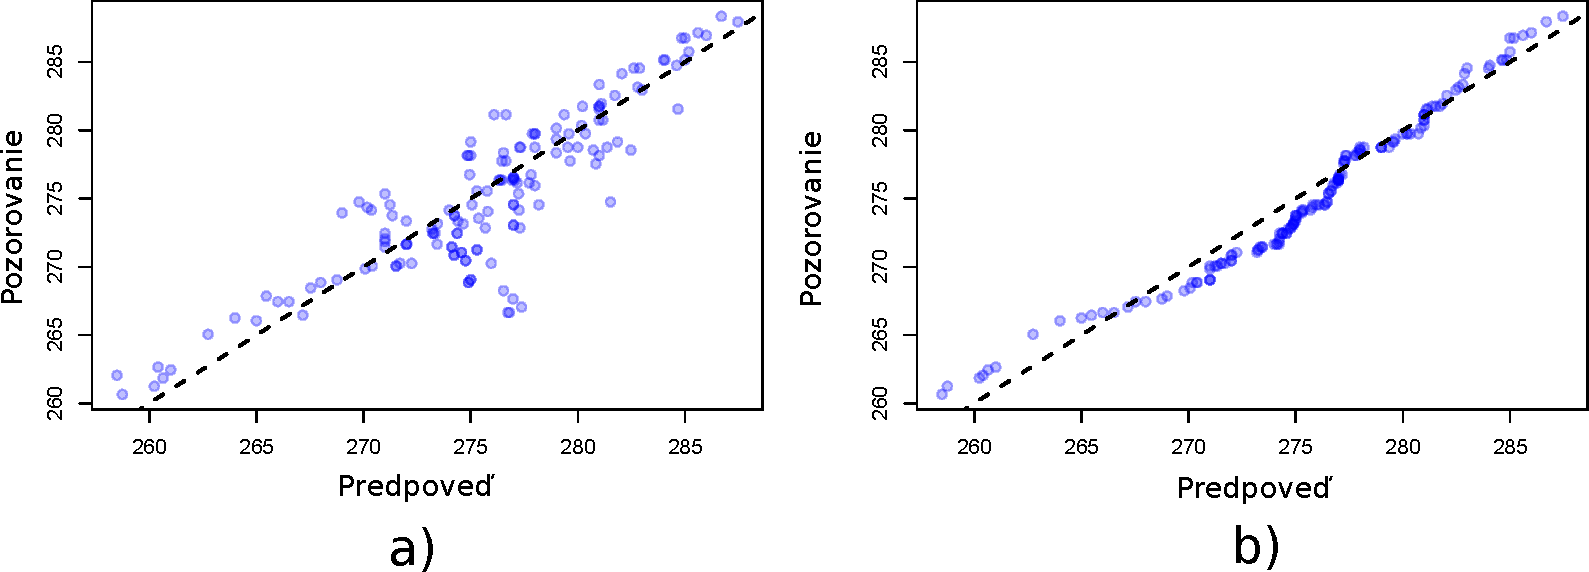
\includegraphics[width = 5.5in]{scattervsqq}
	\caption{Porovnanie bodového grafu a Q-Q grafu pre rovnaké dáta. Oba grafy boli vygenerované v programe EVS \cite{EVS}. a) Bodový graf b) Q-Q graf }
	\label{fig:scattervsqq}
\end{figure}

\subsection{Úloha bodového grafu vo verifikácii}
Úloha bodového grafu a \mbox{Q-Q} grafu vo verifikácii je rovnaká, avšak oba nám dávajú trocha iný pohľad na dáta. Vo všeobecnosti nám tieto dva grafy dávajú informáciu o vzťahu medzi dvoma veličinami, ich korelácii a taktiež aj o ich distribúcii. 

Dôležitým faktorom teda zostáva aké premenné umiestnime na \mbox{$ x $-ovú} a aké na \mbox{$ y $-ovú} os. Vo verifikácii predpovedných modelov počasia sú to zvyčajne predpovede na jednej osi a pozorovania na druhej. Taktiež sa zvyknú robiť dvojice (predpoveď, chyba predpovede), (pozorovanie, chyba predpovede) alebo (čas predpovede, chyba predpovede) a im podobné. V našej aplikácii sme testovali poslednú zo spomenutých dvojíc.

\section{Krabicový diagram}
\label{sec:boxplot}
Krabicový diagram je v anglickej literatúre zvyčajne nazývaný \textit{box plot} alebo na niektorých miestach označovaný tiež ako \textit{box and whisker\footnote{Slovo \textit{whisker} znamená po slovensky fúz, čo naznačuje, že čiary, ktoré spájajú horný a dolný kvartil s hraničnými hodnotami pripomínajú fúzy.} plot}. Odkedy bol prvýkrát publikovaný v roku 1977 \cite{Tukey}, uplynulo už takmer 40 rokov a dnes ho považujeme už za štandardnú techniku ako vizualizovať distribúciu hodnôt kompaktným spôsobom. Na svoju reprezentáciu využíva súbor 5 čísel (tzv. \textit{\mbox{5-number} summary}) \cite{Potter}, ktoré charakterizujú distribúciu dát robustným spôsobom. Tým, že zredukujeme zvyčajne veľkú dátovú množinu na týchto pár hodnôt ušetríme nielen vzácny vizuálny priestor \cite{Wickham}, ale taktiež námahu analytika, ktorý sa snaží preskúmať iba niektoré vybrané charakteristiky. 

\subsection{Konštrukcia krabicového diagramu}

Na zostavenie krabicového diagramu potrebujeme týchto 5 hodnôt: medián, horný a dolný kvartil, maximum, minimum (pozri obrázok \ref{fig:boxplot}). Prvé tri hodnoty sú takzvané kvartily (Q1, Q2, Q3), ktoré rozdeľujú súbor dát na 4 rovnako veľké časti a ďalšie dve sú extrémne hodnoty, ktoré ohraničujú celú dátovú množinu (pozri podsekciu \ref{subsec:qqplot} pre vysvetlenie pojmu kvantil). 

Kvartil Q2 je medián hodnôt a je definovaný rovnako ako v časti \ref{subsec:mad}. Ďalej horný (Q1) a dolný (Q3) kvartil získame ako medián hodnôt pod a nad hodnotou Q2, pričom hodnotu Q2 nezahŕňame do výpočtov. 

Na obrázku \ref{fig:boxplot} vidíme, že krabica v grafe určuje pozície horného a dolného kvartilu, zatiaľ čo vnútro krabice znázorňuje takzvané \textit{IQR}. Táto skratka označuje \textit{interquartile range}, čo sa dá preložiť ako \textit{medzikvartilový rozsah}. IQR definujeme ako rozdiel kvartilov Q3 a Q1:
\[
IQR = Q3 - Q1
\]
IQR nám hovorí o vzdialenosti týchto dvoch kvartilov, preto nám môže byť tento vzorec na pohľad podozrivý, keďže sa javí, že IQR by mohlo nadobúdať aj záporné hodnoty. My však vieme z definície Q3 a Q1, že $ Q3 > Q1 $ a ich rozdiel je teda vždy nezáporný (Hovoríme o rozdiele Q3 od Q1, tak ako je definované IQR).

Malú obmenu pôvodného návrhu krabicového diagramu od Tukeyho, vidíme na obrázku \ref{fig:boxplot} b), kde malé bodky znázorňujú hodnoty nazývané \textit{outlier}, teda hodnoty ležiace ďaleko od hlavného dátového tela, a hviezdička v strede diagramu určuje priemer hodnôt. Môžme si všimnúť, že konce čiar vychádzajúcich z boxu nemôžu byť extrémy celej množiny dát, ale sú iba extrémami vypočítaných z dát bez \mbox{\textit{outlier}-ov}.

Otázkou zostáva ako určiť, ktorá hodnota je \textit{outlier} a ktorá nie je. Na zodpovedanie tejto otázky sa využíva už spomínaný rozsah IQR. Pomocou neho sa definujú hranice \textit{inner fences} ($f_{1}, f_{2}$) a \textit{outer fences} ($F_{1}, F_{2}$), za ktorými hovoríme už o \mbox{\textit{outlier}-och} alebo o ďalekých \mbox{\textit{outlier}-och} \cite{Schwertman}. Definované sú nasledovne:
\\
\[f_{1} = Q1 - c \times IQR\]	
\[f_{2} = Q3 + c \times IQR\]
\[F_{1} = Q1 - C \times IQR\]
\[F_{2} = Q3 + C \times IQR\]

Konštanty $ c $ a $ C $ sú v niektorých zdrojoch definované rôzne. Najčastejšie sa však vyskytujú hodnoty $ c = 1.5 $ a $ C = 3$, tak ako ich určil pôvodný autor krabicového diagramu \cite{Tukey}.

\begin{figure}
	\centering
	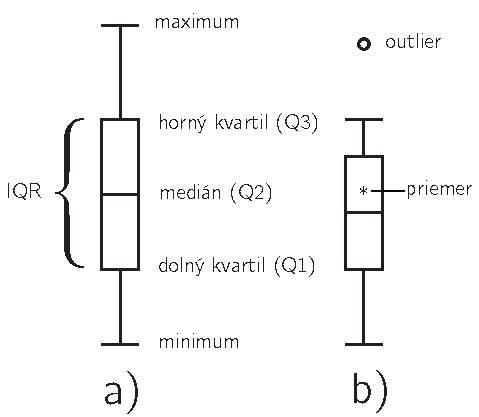
\includegraphics[width = 3.5in]{boxplot}
	\caption{Pôvodný návrh krabicového diagramu, ako bol prezentovaný v práci \textit{Exploratory Data Analysis}(1977) \cite{Tukey} }
	\label{fig:boxplot}
\end{figure}


\subsection{Ďalšie variácie krabicového diagramu}

Popularita krabicového diagramu nevyhnutne viedla k jeho vývoji a modifikáciám. Môžeme hovoriť o dvoch druhoch modifikácií. Jednak \textit{syntaktickej} (vizuálnej), kedy sa zachovávajú všetky vlastnosti a informácie ako v pôvodnom diagrame, len sa menia vizuálne prvky grafu. A modifikácii \textit{sémantickej} pridaním ďalšej popisnej informácie do grafu, čo má na záver vplyv aj na jeho vizuálnu stránku.


\begin{figure}
	\centering
	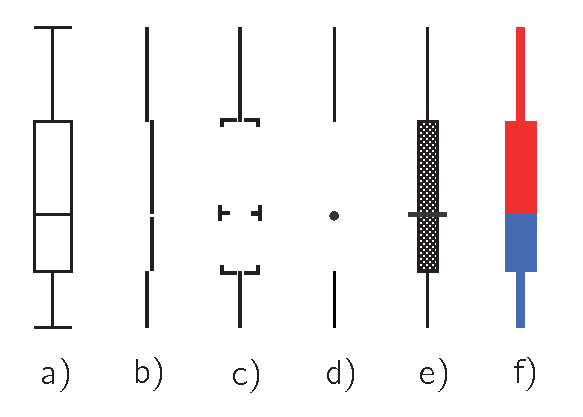
\includegraphics[width = 4in]{boxplot2}
	\caption{ a) Klasický krabicový diagram  b-f) Vizuálne variácie krabicového diagramu \mbox{b-c) 2 variácie pre kvartilový graf \cite{Tufte83}} \mbox{c) Skrátený krabicový diagram \cite{VisualSummaryPotter}} \mbox{e) \mbox{Range-bar} chart \cite{Spear}} \mbox{f) Farebná variácia \cite{Carr}}  }
	\label{fig:boxplotmodif1}
\end{figure}


\paragraph{}
{\large \textbf{\textit{N}}}a obrázkoch \ref{fig:boxplotmodif1} b-f) môžme vidieť niektoré vizuálne variácie krabicového diagramu. Vznik prvých troch motivovala snaha maximalizovať takzvaný \textit{data-ink} \cite{Tufte83}, teda množstvo atramentu alebo počet pixlov, ktoré zodpovedajú nejakým dátam. Autori sa teda snažili čo najviac znížiť počet vizuálnych prvkov a ponechať len tie, ktoré skutočne nesú nejakú informáciu. 

Na obrázku \ref{fig:boxplotmodif1} b) a c) vidíme dve z viacero riešení navrhnutých v knihe \textit{The Visual Display of Quantitative} \cite{Tufte83}, ktoré autor nazýva \textit{kvartilový graf}. Preceptuálne štúdie \cite{Stock} však ukázali, že tieto variácie sú výrazne menej presné ako originálny návrh.

Návrh d) ukazuje skrátený krabicový diagram \cite{VisualSummaryPotter}, ktorý sa taktiež snažil zredukovať množstvo okupovaného vizuálneho priestoru. Rozdielom je však to, že jeho účelom nie je existovať samostatne, ale ako súčasť \mbox{\textit{summary plot}-u}, ktorý zahŕňa histogram a ďalšie glify znázorňujúce informácie ako priemer, štandardná odchylka alebo koeficient asymetrie.

Obrázok \ref{fig:boxplotmodif1} e) znázorňuje predchodcu krabicového diagramu \textit{range} graf alebo tiež nazývaný \mbox{\textit{range-bar}} graf, ktorého autorkou je Mary Eleanor Spear \cite{Spear}.

Ako posledný príklad vizuálnej modifikácie uvádzame pridanie farieb do krabicového diagramu. Táto farebná variácia uchováva tvar diagramu, avšak časť nad mediánom je zafarbená inou farbou ako hodnoty pod. Autori článku odporúčajú červenú a modrú farbu, tak ako na obrázku \ref{fig:boxplotmodif1} f). Cieľom tohto prístupu bolo chápať krabicový diagram ako jednu percepčnú jednotku a nahradiť 5 symbolov jedným, čím sa mala znížiť námaha pozorovateľa pri analýze a taktiež uľahčiť porovnávanie viacerých diagramov navzájom. 

\begin{figure}
	\centering
	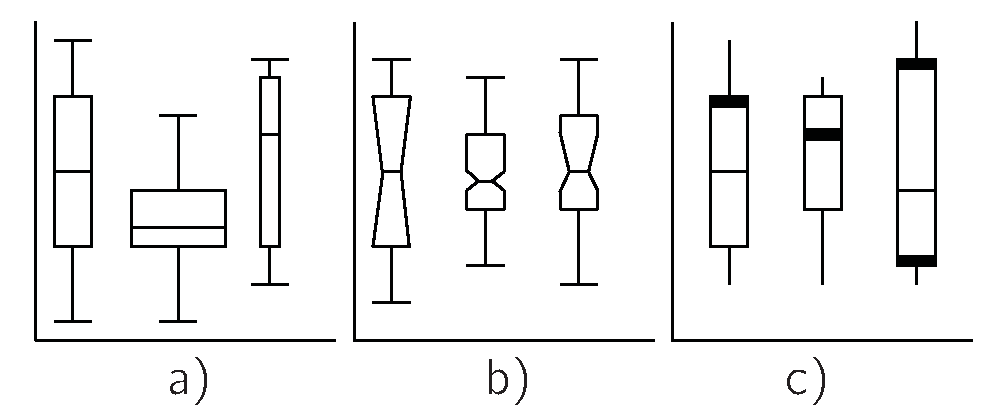
\includegraphics[width = 6in]{boxplot3}
	\caption{Krabicové diagramy s pridanou informáciou a) Krabicový diagram s variabilnou šírkou \cite{McGill} b) Vrúbkovaný krabicový diagram \cite{McGill} c) Krabicový diagram s informáciou o šikmosti dát \cite{Chamnein}}
	\label{fig:boxplotmodif2}
\end{figure}

\paragraph{}
{\large \textbf{\textit{K}}}rabicový diagram umožňuje svojim vzhľadom zakódovanie ďalšej informácie do grafu. Na obrázku \ref{fig:boxplotmodif2} vidíme aspoň niektoré najčastejšie úpravy krabicového diagramu, ktoré dopĺňajú dodatočnú informáciu zmenou parametrov vizuálnych prvkov krabicového diagramu.

Len rok po oficiálnom publikovaní krabicového diagramu vznikol článok \cite{McGill}, ktorý zhŕňa jeho tri najčastejšie používané modifikácie, z ktorých prvé dve môžme vidieť na obrázkoch \ref{fig:boxplotmodif2}a) a \ref{fig:boxplotmodif2}b) a tretí je ich kombináciou. V prvom prípade sa využíva šírka boxu na zakódovanie veľkosti množiny, ktorú skrýva za sebou diagram. Takýto graf sa nazýva \textit{Krabicový diagram s variabilnou šírkou}.  
V druhom prípade ide o takzvaný \textit{Vrúbkovaný krabicový diagram}. V tomto grafe sú pridané \textit{vrúbky}, ktoré zhruba naznačujú ako výrazné sú rozdiely v miere spoľahlivosti rôznych dátových množín. 

V niektorých prípadoch krabicový diagram zakrýva skutočný tvar dát, teda jeho šikmosť alebo modalitu, keďže jeho vzhľad nabáda k tomu, aby si užívateľ myslel, že sú dát zacentrované na stred a unimodálne. V práci s názvom \textit{Can the Box Plot be Improved?} \cite{Chamnein} autor uvádza príklad kedy skutočne rôznorodé dáta generujú rovnaký krabicový diagram. Tento problém rieši elegantným a čistým spôsobom pridaním hrubej čiary na základe koeficientu asymetrickosti $ \gamma $. Na obrázku \ref{fig:boxplotmodif2}c) môžme vidieť zľava asymetrické dáta, na stred zarovnané dáta a bimodálne dáta.

Krabicový diagram umožňuje mnoho ďalších rozšírení napríklad pridaním informácie o hustote dát (histogramový krabicový diagram, vázový diagram \cite{HistVasePlot} , huslový diagram \cite{ViolinPlot}), rozšírením pre viacrozmerné dáta (vrecový graf \cite{Bagplot}, 2D krabicový diagram \cite{Boxplot2D} ) alebo zobrazením hodnôt v inej súradnicovej sústave (napríklad polárnej - vejárový graf \cite{FanChart}). Opis týchto techník je však nad rámec tejto práce, preto ho tu ani nebudeme uvádzať.

\subsection{Úloha krabicového diagramu vo verifikácii}

Ako sme spomenuli v úvode tejto sekcie, vo všeobecnosti je úlohou krabicového diagramu zobraziť distribúciu dát v kompaktnom tvare a teda slúži na rýchle porovnanie distribúcií viacerých skupín dát.
Pri verifikácii predpovede spojitých premenných sa používa na viacero účelov a my tu spomenieme len niekoľko z nich. 

V prvom rade ide o porovnanie distribúcie predpovedí s distribúciou pozorovaní za istý časový interval. V takomto prípade máme vedľa seba iba dva krabicové diagramy, ktoré navzájom porovnávame. Použitie krabicového diagramu v takomto prípade, kedy jeden graf pozostáva iba z niekoľkých (2 až 4) krabicových diagramov považujeme za zbytočné. Pri takomto počte nie je potreba na redukciu vizuálnych prvkov a existujú lepšie techniky na vizualizáciu distribúcie, ktoré sprostredkúvajú viacej informácie a teda môže byť analýza efektívnejšia. 

Ďalším použitím je porovnanie distribúcie chýb predpovedí, či už pre rôzne merania, konkrétne predpovedané časy, rôzne predpovedné modely a podobne. Tu považujeme použitie krabicového diagramu za opodstatnené, keďže ide zväčša o porovnávanie väčšieho množstva distribúcií, a tak je potrebná jeho jednoduchosť, čitateľnosť, kompaktnosť a iné jeho vlastnosti.

\section{Histogram}
\label{sec:histogram}
Ďalším veľmi bežným spôsobom, ako vizualizovať distribúciu dát je pomocou \textit{histogramu}, ktorého existencia sa datuje do roku 1895, kedy ho uviedol vo svojej práci Karl Pearson \cite{histogram}. Histogram využíva veľmi jednoduchú myšlienku vizualizovať frekvencie hodnôt ako stĺpce rôznej výšky, ktorá sa v priebehu histórie analýzy dát ukázala ako veľmi užitočná.

\subsection{Konštrukcia histogramu}
Konštrukcia histogramu je pomerne jednoduchá. V prvom rade potrebujeme rozdeliť interval hodnôt na disjunktné podintervaly rovnakej dĺžky. Na vygenerovanie týchto intervalov využíva autor diagramu počiatok $ O $ a veľkosť intervalu $ w $. Prvý interval je $ \langle O, O + w) $ a všetky nasledujúce vzniknú posúvaním intervalu o dĺžku $ w $ v kladnom smere. Ďalej pre každý takto vzniknutý interval vypočítame koľko hodnôt doň spadá. Potom už môžme vykresliť jednotlivé stĺpce pre každý interval ako obdĺžniky so šírkou $ w $ a výškou, ktorá sa určí na základe početnosti hodnôt pre daný interval. Na obrázku \ref{fig:histogram} môžeme vidieť takýmto spôsobom vygenerovaný histogram.

\begin{figure}
	\centering
	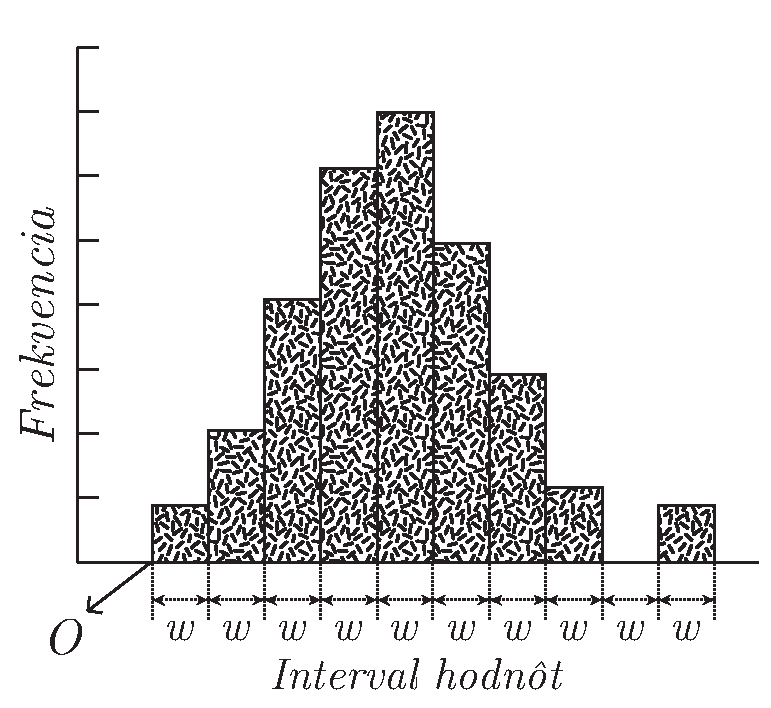
\includegraphics[width = 2.5in]{histogram}
	\caption{ Histogram }
	\label{fig:histogram}
\end{figure}

Z vyššie popísaného postupu a rovnako aj z obrázka \ref{fig:binsizehistogram} môžme vidieť, že konštrukcia histogramu závisí od zvoleného počiatku $ O $, no v prvom rade od zvolenej veľkosti intervalu $ w $. Z tohto dôvodu vzniklo mnoho prístupov, ktoré sa snažia optimalizovať $ w $, tak aby sa získal optimálny histogram. Optimálny histogram $ h(x) $ je taký, ktorý minimalizuje integrovanú strednú kvadratickú chybu (\textit{MISE}) vzhľadom na pôvodnú funkciu hustoty $ f(x) $. Túto chybu vypočítame takto: $ MISE = \int (h(x) - f(x))^2 dx $. 

Jedným z príkladov, ktorý toto využíva je algoritmus na generovanie optimálnej hodnoty $ w $, ktorý navrhol \textit{Shimazaki} a \textit{Shinomoto} \cite{OptBinSize}. Autori algoritmu požívajú dekompozíciu MISE na vytvorenie cenovej funkcie $ C_{n}(w) $ pre dĺžku intervalu $ w $:
\[
	C_{n}(w) = \frac{2\bar{k} - v}{(nw)^2}
\]
kde $ n $ je počet všetkých hodnôt množiny, $ \bar{k}$ je priemerný počet hodnôt v jednom intervale a $ v $ je variancia počtu hodnôt v intervaloch. Priebeh algoritmu je potom už len taký, že generuje postupne rôzne $ w $, kým nenájde také s najmenšou cenou $ C_{n}(w) $. 

\begin{figure}
	\centering
	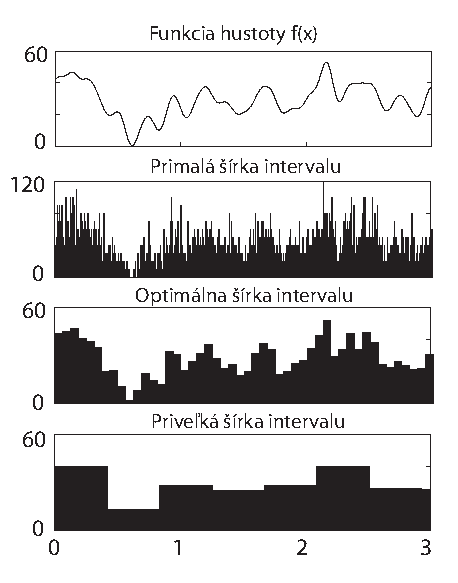
\includegraphics[width = 3.7in]{binsizehistogram}
	\caption{ Porovnanie rôznych dĺžok intervalov. Obrázok je upravený z pôvodného článku \cite{OptBinSize} }
	\label{fig:binsizehistogram}
\end{figure}

 
\subsection{Úloha histogramu vo verifikácii}
Ako sme už spomenuli, primárna úloha histogramu je detailná vizualizácia distribúcie dát. Vzhľadom k vysokej úrovni detailu, nie je jednoduché porovnávanie mnoho histogramov súčasne, tak ako to bolo u krabicového diagramu. Z tohto dôvodu sa zvyčajne v praxi porovnáva navzájom len niekoľko rôznych histogramov. Vo verifikácii histogramy slúžia na porovnanie distribúcie predpovedí a pozorovaní. Porovnávanie stĺpcov histogramov sa robí buď v dvoch rôznych diagramoch umiestnených vedľa seba alebo v jednom diagrame, kde sa stĺpce patriace k sebe umiestnia pri seba a rozdielne zafarbia, aby ich bolo možné ľahšie rozlíšiť.

\section{Čiarový diagram}
\label{sec:linegraph}
\textit{Čiarový diagram} je najjednoduchší spôsob ako vizualizovať jednorozmerné dáta. Využíva sa najmä na vizualizáciu spojitej premennej, keďže čiara narozdiel od bodov podporuje vizuálny dojem spojitosti. Pôvod čiarového diagramu sa datuje do prapočiatkov vizualizácie informácií. Jeho autorom je zakladateľ grafických metód v štatistike William Playfair, ktorý objavil 4 typy diagramov medzi, ktorými bol aj čiarový diagram v roku 1786 \cite{HistoryOfInfoVis}.

\subsection{Konštrukcia čiarového diagramu}
Pri konštrukcii čiarového diagramu sa hodnoty z množiny zobrazia v karteziánskej sústave ako body a jednotlivé dvojice susedných bodov sa následne pospájajú čiarou. Na obrázku \ref{fig:linegraph} môžme vidieť príklad čiarového grafu vytvoreného týmto postupom.

Čiarový graf poskytuje rôznorodé úpravy, ktoré pridávajú ďalšiu informáciu do grafu alebo zlepšujú niektoré vizuálne vlastnosti. Napríklad je možné upravovať šírku, tvar alebo farbu čiary, pridávať ďalšie čiary do grafu, zvýrazniť jednotlivé body pre dané hodnoty, použiť iný typ interpolácie medzi bodmi (zvyčajne sa používa lineárna interpolácia) a podobne.

\subsection{Úloha čiarového diagramu vo verifikácii}
Vo verifikácii je účelom čiarového diagramu vizualizácia časových radov. Na \mbox{$ x $-ovej} osi zvykne byť časový interval s konkrétnymi dátumami predpovedí alebo hodiny predpovede. Rozdiel medzi nimi je ten, že konkrétny dátum je v histórii iba raz, zatiaľ čo model predpovedá pravidelne, takže predpovedné hodiny môžu byť rovnaké pre rôzne dátumy. Na \mbox{$ y $-ovej} osi teda bývajú buď jednotlivé hodnoty chýb alebo pre viacero hodnôt vypočítané štatistiky ako boli spomenuté v časti \ref{sec:errormeasurement}.
 

\begin{figure}
	\centering
	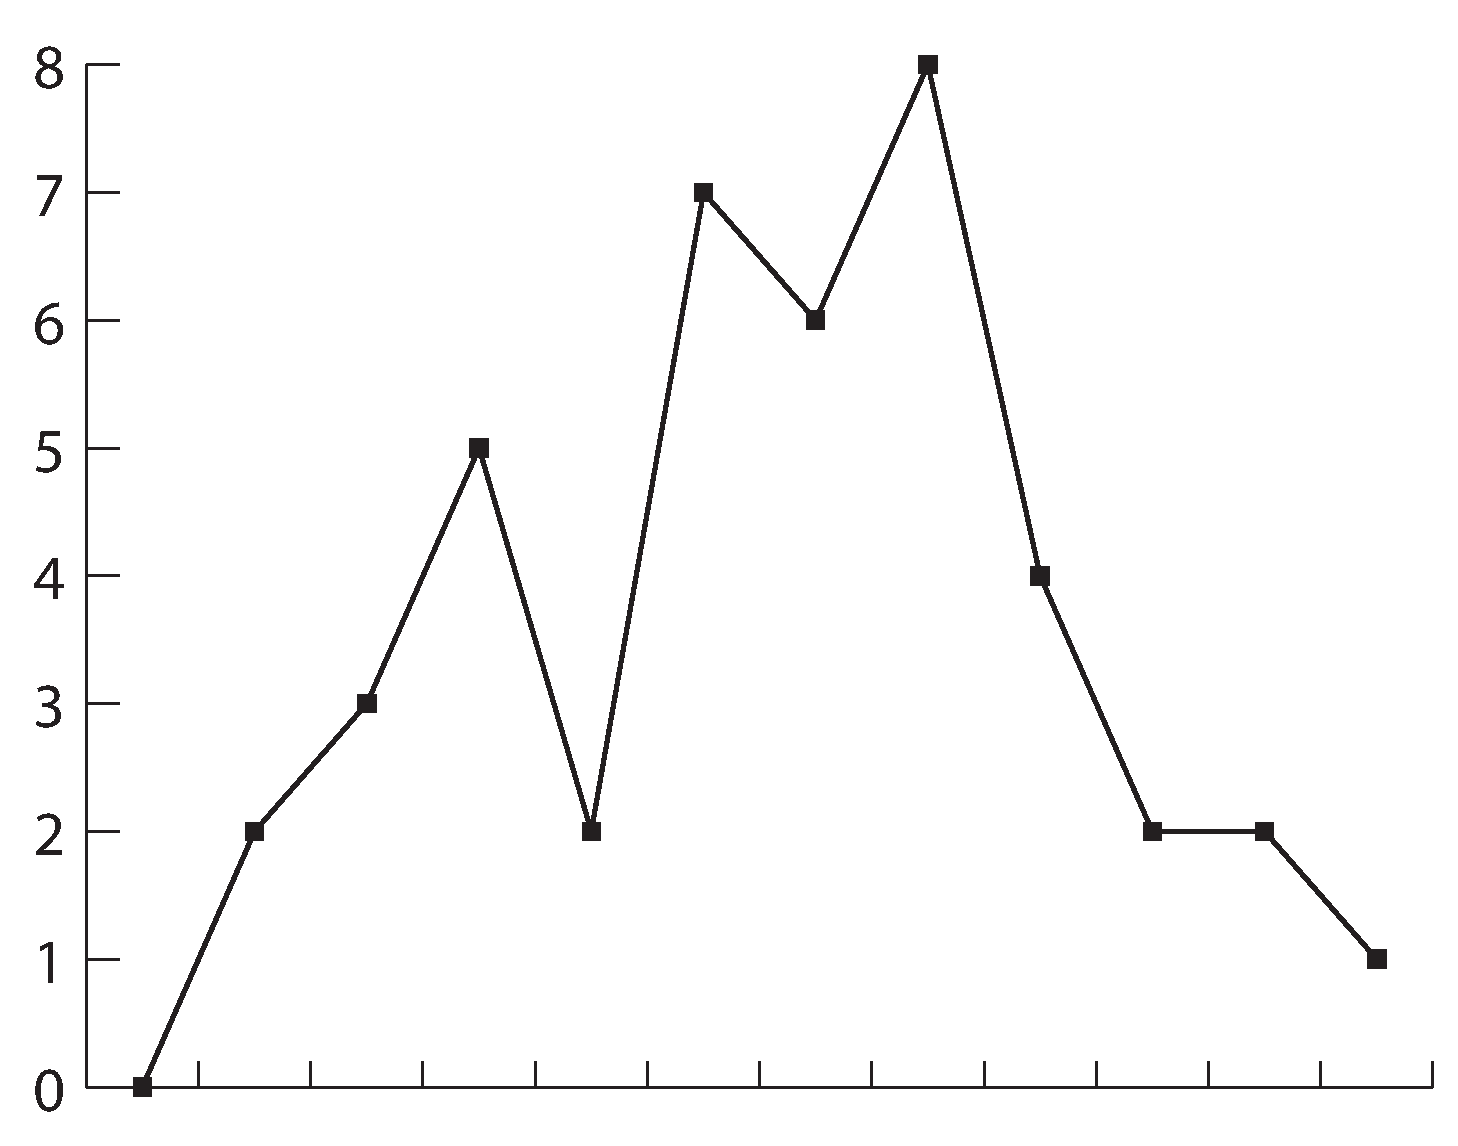
\includegraphics[width = 3in, height=1.5in]{linegraph}
	\caption{Príklad čiarového grafu vygenerovaného v programe Adobe Illustrator}
	\label{fig:linegraph}
\end{figure}

\section{Taylorov diagram}
\textit{Taylorov diagram} bol špeciálne navrhnutý pre verifikáciu modelov počasia, ktorého autorom je Karl. E. Taylor \cite{Taylor}. Podľa slov autora úlohou diagramu je štatistické zhrnutie, ako dobre si dátové vzory zodpovedajú v zmysle troch metrík: koeficient korelácie, stredná kvadratická chyba a smerodajná odchýlka. Použitie taylorovho diagramu nie je tak časté ako pri predchádzajúcich vizualizačných technikách, možno aj z dôvodu horšej čitateľnosti grafu a taktiež nemá takú veľkú tradíciu v štatistike, ako predošlé techniky. Podobnú snahu zobraziť tri štatistiky súčasne v jednom grafe mal aj Boer a Lambert vo svojom BLT diagrame \cite{Boer}. Tento typ grafu je veľmi podobný taylorovmu grafu, a keďže jeho použitie je ešte zriedkavejšie, tak sa mu v tejto práci nebudeme venovať.
  
\subsection{Konštrukcia taylorovho diagramu}
Taylorov graf porovnáva jednu alebo viacero dátových množín ($ f $) s jednou referenčnou množinou $ r $. Označme si hodnoty v porovnávanej množine $ f_{n} $ a s nimi spárované referenčné hodnoty $ r_{n} $, ktoré sú definované na $ N $ diskrétnych bodoch (napríklad v čase alebo priestore). Ako sme už spomenuli, taylorov graf vizualizuje 3 štatistiky súčasne, na čo využíva ich vzájomný geometrický vzťah. Týmito štatistikami sú: koeficient korelácie $ R $, centrovaná stredná kvadratická chyba $ E' $ a smerodajné odchýlky $ \sigma_{f} $ a $ \sigma_{r} $ pre $ f, r $.  Vzorce na výpočet sú nasledovné:
\[
	R = \dfrac{\frac{1}{N} \sum_{n=1}^{N}(f_{n} - \bar{f})(r_{n} - \bar{r})  }{\sigma_{f}\sigma_{r}}
\]
, kde $ \bar{f} $ a $ \bar{r} $ sú priemerné hodnoty daných množín.
\[
	E' = \sqrt{\frac{1}{N} \sum_{n=1}^{N}[(f_{n} - \bar{f}) - (r_{n} - \bar{r})]^2 }
\]
Pre pripomenutie chceme upozorniť, že nejde o strednú kvadratickú chybu, ktorá bola spomenutá v časti \ref{sec:errormeasurement}, ale o \textit{centrovanú} strednú kvadratickú chybu, ktorá je relatívna k stredu, teda priemeru skúmaných množín.

Rovnako pre $ \sigma_{f} $ aj $ \sigma_{r} $ je výpočet nasledovný:
\[
\sigma_{x} = \sqrt{\frac{1}{N} \sum_{n=1}^{N}[(x_{n} - \bar{x})]^2 }
\]

\begin{figure}
	\centering
	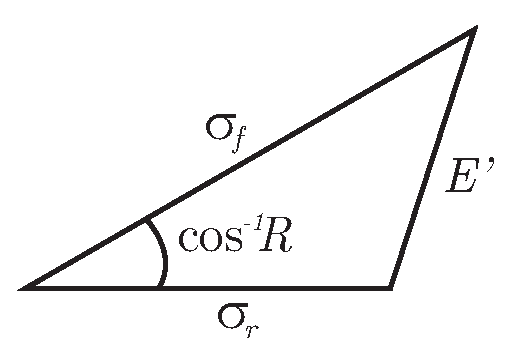
\includegraphics[width = 2.8in]{taylortriangle}
	\caption{ Geometrický vzťah pre popisné štatistiky $ R, E', \sigma_{r}, \sigma_{f} $ }
	\label{fig:gemrelationship}
\end{figure}

Kľúčovým bodom v konštrukcii diagramu je, že s využitím týchto troch respektíve štyroch štatistík môžme skonštruovať nasledovný vzťah:
\[
	E^{\prime2} = \sigma_{f}^{2} + \sigma_{r}^{2} - 2\sigma_{f}\sigma_{r}R
\]
, ktorý sa nápadne podobá na kosínusovú vetu:
\[
	a^{2} = b^{2} + c^{2} - 2bc\cos\alpha 
\]
, kde $ a, b $ a $ c $ sú dĺžky strán trojuholníka a uhol $ \alpha $ je protiľahlý uhol pre stranu $ a $. Geometrický vzťah pre $ R, E', \sigma_{f} $ a $ \sigma_{r} $ je zobrazený na obrázku \ref{fig:gemrelationship}. Ako vidíme na obrázku \ref{fig:taylordiagram}, jedna dátová množina sa pomocou týchto troch spomenutých hodnôt a vyššie uvedeného geometrického vzťahu zobrazí na grafe s polárnymi súradnicami. Azimutálna pozícia bodu nám hovorí o korelačnom koeficiente medzi množinami, preto sa vždy referenčný bod nachádza v najnižšej úrovni grafu, kde je korelácia rovná jednej. Vzdialenosť od počiatočného bodu $ 0 $ nám udáva smerodajnú odchýlku $ \sigma $ a vzdialenosť od referenčného bodu udáva centrovanú RMSE $ E' $. Pre jednoduchšie odčítavanie hodnôt sa pridávajú aj označené radiálne čiary jednak od bodu $ 0 $, ale aj od referenčného bodu, ktoré sa však v praxi zvyknú vynechávať.

\begin{figure}
	\centering
	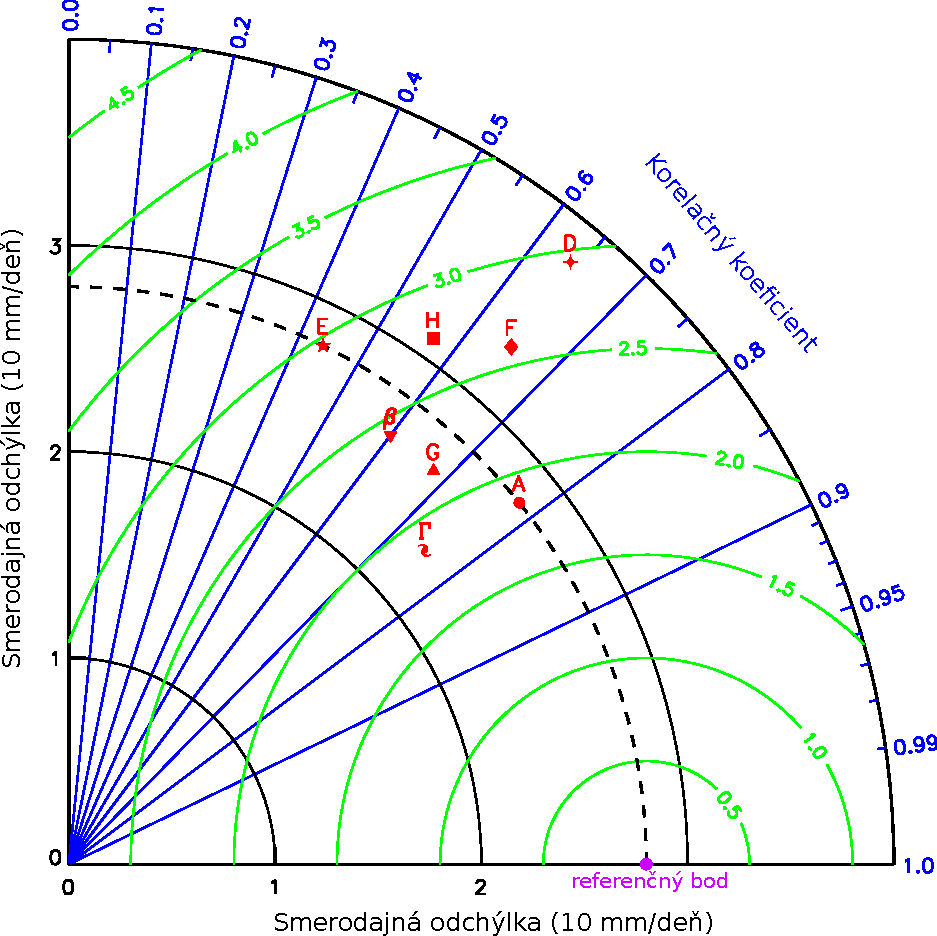
\includegraphics[width = 3.5in]{taylordiagram}
	\caption{ Taylorov diagram \cite{Taylor} }
	\label{fig:taylordiagram}
\end{figure}

Popísaným spôsobom vytvoríme základný taylorov diagram, ktorý však ponúka niekoľko modifikácií \cite{TaylorPrime}, z ktorých niektoré používané spomenieme:

\begin{singlespacing}
\begin{itemize} 
	\item Diagram môže byť rozšírený o ďalší kvadrant vľavo, na zobrazenie zápornej kolerácie 
	\item Štatistiky porovnávaných hodnôt môžu byť normalizované pomocou štatistík referenčných, čím dosiahneme, že na jednom diagrame možno zobraziť rôzne jednotky veličín.
	\item Izočiary sa vynechávajú, aby bolo možné lepšie vidieť zobrazené body.
	\item Pri porovnávaní výsledkov z viacerých verzií predpovedných modelov sa zvykne nakresliť šípka medzi týmito bodmi, aby bolo lepšie vidieť vzťah medzi nimi.
	\item Miera $ E' $ môže byť nahradená inou. Niektoré príklady mier možno nájsť v Taylorovom článku \cite{Taylor}
	\item Do grafu je možno pridať ďalšiu informáciu modifikovaním vizuálnych vlastností bodu podobne ako v bodovom diagrame. Jedným z príkladov je zobrazenie percentuálnej priemernej chyby pomocou rôznych symbolov.
\end{itemize}
\end{singlespacing}



\subsection{Úloha taylorovho diagramu vo verifikácii}
Tento typ diagramu bol priamo navrhnutý pre účely verifikácie predpovedných modelov počasia. Hlavným účelom diagramu je porovnávanie výkonu viacerých modelov alebo tiež jedného modelu s rôznymi nastaveniami parametrov. 

Taylorov diagram skrýva dáta pod komplikovaný matematický model, ktorý nám poskytuje 3 vyššie popísané charakteristiky dát na vizualizáciu. Ak sa k tomu pridáva fakt, že diagram umožňuje iba jednu referenčnú dátovú množinu, tak použitie tohto diagramu je značne obmedzené. Využitím spomínaných troch charakteristík taktiež výrazne strácame pohľad na detail dát, ale na druhej strane nám to umožňuje jednoduché porovnávanie pomerne veľkých a komplikovaných množín na malom priestore. 

Ďalšou slabinou je, že charakteristika $ E' $ sa počíta ako centrované RMSE, ktoré je relatívne vzhľadom na stred teda priemernú hodnotu dátovej množiny. Tento fakt implikuje to, že centrované RMSE nemá jednu dôležitú vlasnosť, ktorú naopak klasické RMSE má. Touto vlastnosťou je, že čím je RMSE bližšie k nule, tým podobnejšie sú aj dátové množiny. Keďže štatistická charakteristika $ E' $ nemá túto vlastnosť, tak nám euklidovská vzdialenosť skúmaného bodu od referenčného nedáva dobrú informáciu o podobnosti dvoch množín a môže pôsobiť dezinformačne.